% !TeX spellcheck = en_GB
\documentclass[../summary.tex]{subfiles}

\begin{document}
	
	\section{Social and economic inequality}
	
	\subsection{Study guide}
	
	Module 11 sketches basic insights into inequality both within and between countries. Make sure to understand:
	\begin{itemize}
		\item Inequality as a multi-dimensional concept: you can’t express inequality in only a single number or indicator
		\item Sources of inequality (according to philosophical literature): fate, personal choice, social circumstances + which is considered problematic
		\item Inequality between countries versus inequality within countries
		\item Main criticism of Philip Alston against the World Bank’s 
		definition of the International Poverty Line
		\item Different drivers of inequality:
		\begin{itemize}
			\item What the theory says about the effects of neoliberal globalization on the evolution of inequality, and why reality proved partially different
			\item The increasing concentration of capital: understand the differences between wealth inequality and income inequality. Understand what r > g means in this respect, and how it can influence the way societies function (concentration of power, land robbing)
			\item environmental and climate disruption: poor people often live in the most polluted areas and are at the same time more often dependent on their natural environment (grazing, farming,…)
		\end{itemize}
		\item Reasons why we should be concerned about inequality (also beyond the mere ethics): link with human rights, link with economic development, link with environmental sustainability, societal well-being, political stability
		\item Policy solutions (and the link to the drivers)
		\item Kate Raworth’s model of the doughnut economy 
	\end{itemize}
	
	\subsection{Inequality as a multi-dimensional concept}
	
	Inequality is all about some people having more than others and refers to rankings on quantitative scales. It is very difficult to pinpoint what we should use as a yardstick for such a scale. We can use financial measures, but then there are still lots of possibilities. If we take the net disposable income, we need to consider differences in size and composition of households and even if we balance this scale, we need to consider that each household can have different assets. But there is more to it: the living standard of a person or household also depends on their access to collective services like education or culture, their schooling and skills, their health, their network of friends, their participation in social life... All these items can be considered resources – material as well as immaterial. In other words, inequalities are multidimensional.  
	
	\subsection{Sources of inequality}
	
	In the philosophical literature, a distinction is usually made between three sources of inequality: fate, personal choice, and socio-economic environment.
	\\\\
	Firstly, \textbf{fate} refers to inequalities that are due to some natural condition beyond the power of men: the most typical example here is differences in innate abilities. Some people are born very talented, others are not. Even the most democratic education systems will not wipe out these differences. Society could try to compensate for their income differences, but not their differences in learning abilities and skills. The same argument could apply to innate differences in health, psychological condition etc. 
	\\\\
	Secondly, \textbf{personal choice} may affect inequalities, simply because people have freedoms and diverse preferences: some are workaholics while others are Zen; some hate to study while others cannot get enough of it; some are entrepreneurial while others are epicureans. It is impossible to impose uniform rules as straitjackets to avoid these inequalities, nor even the differences in material welfare that go in pair with them.
	\\\\
	It is the third source of inequalities, \textbf{social circumstances}, which is commonly seen as problematic. You cannot choose the cradle in which you are born nor the wealth or skin colour of your parents, and yet all too often those conditions determine your odds in life to a large extent. The overwhelming majority of the population would agree that neither your socio-economic or ethnic background, nor even the region where you grow up can be accepted as legitimate sources of inequality. These are beyond the scope of individual choice, but within the scope of collective choice. Therefore, from a moral point of view, society (and the government) are deemed responsible for the minimization of these sources of inequality. 
	
	\subsection{Inequality between versus within countries}
	
	Inequality between countries stems from the fact that there is a difference between the wealth of rich (First World) countries and developing countries. Within these countries, there is also inequality between people. This inequality can have a lot of reasons, such as social status or education level.
	
	\subsection{Main criticism of Philip Alston}
	
	There are 7 key takeaways from Philip Alston's criticism:
	\begin{enumerate}
		\item \textbf{There has been a ‘dramatic and longstanding’ neglect and ‘downplaying’ of extreme poverty} by many governments, economists, and human rights advocates.
		\item \textbf{The claim that extreme poverty is nearing eradication is unjustified.}
		\item  \textbf{Using a more defensible IPL generates a radically different picture.}
		\item \textbf{The impact of COVID-19 will be long-lasting.}
		\item \textbf{While the SDG process has been a ‘game-changer’ in important ways} and has been used to very good effect in many settings ‘promoting awareness, galvanizing support, and framing the broader debate around poverty reduction’ and often providing ‘the only available entry point for discussions of contentious issues’, 5 years after their adoption it is time to acknowledge their failings and the ‘deeply disappointing results to date and a range of new challenges.’
		\item \textbf{‘Continued large-scale global poverty is incompatible with the human right to an adequate standard of living, and the right to life alongside the right to live in dignity.} The failure to take the necessary steps to eliminate it is a political choice and one that leaves firmly in place discriminatory practices based on gender, status, race, and religion, designed to privilege certain groups over others.’ 
		\item \textbf{‘To avoid sleepwalking towards assured failure while pumping out endless bland reports, new strategies, genuine mobilization, empowerment, and accountability are needed.} Recalibrating the SDG framework itself in response to fundamentally changed circumstances is an urgent first step.’
	\end{enumerate}
	
	\subsection{Drivers of inequality}
	
	The three biggest drivers of inequality that played a key role in the past decades and still mater today are the neoliberal globalization model, the increasing concentration of capital, and environmental and climate disruption.
	\newpage
	The \textbf{neoliberal globalization} has a strong economic underpinning, based on free trade as an engine of global prosperity. In open competitive world markets, whoever can produce a good or service cheaper than others will see their exports grow. Likewise, whenever imported goods are cheaper than those that are produced locally, consumers will benefit from lower prices under free trade and see their purchasing power increase. In a diverse and globalized world, all countries will tend to specialize in their most competitive sectors and reduce their production of other ones, which results in efficiency gains, economic growth and less poverty on a global scale. Rich countries will tend to specialize in capital- and knowledge-intensive sectors such as pharmaceuticals or financial services, while developing countries have an advantage when specializing in sectors that use their abundant low-qualified labour, such as agriculture or textiles. The theory also predicts a downside, however: namely, greater inequality in rich countries. Their specialization mainly benefits capital owners and the highly educated, while the imports or outsourcing of low-skilled-labour-intensive activities undermine the job opportunities and incomes of their own low-skilled people. In contrast, developing countries would only benefit from free trade because they can specialize in labour-intensive sectors, which employ many low-skilled people. This should lead to a more equal income distribution in the South. This is the theory of the effects of neoliberal globalization on the evolution in inequality. In reality, there are also developing (mainly Latin-American) countries where poverty and inequality have increased. The reason for this is that free trade can only thrive in a context of equality between the parties involved. This assumption obviously does not fit with reality. Rich countries have used their power to negotiate unbalanced trade agreements. They have pressurized developing countries to open up their markets, while protecting their own markets in the North.
	\\\\
	 Next, we look at the \textbf{increasing concentration of capital}. First we must understand the difference between income inequality and wealth inequality. Income is a ‘flow’ concept: it is a revenue linked to a particular time period (e.g. a year). Income inequality refers to the unequal distribution of income among a population. It focuses on the disparity in earnings or income levels among individuals or households in a particular area or society. Wealth, on the other hand, is a ‘stock’ concept, measured at a point in time (e.g. December 31st). Wealth inequality pertains to the uneven distribution of assets and possessions (wealth) within a population. Wealth includes not only income but also property, savings, investments, and other forms of accumulated assets. Figure \ref{fig:income-versus-wealth} depicts the difference between income and wealth inequality. In ‘normal times’, the return to capital assets (r) appears to systematically exceed the rate of economic growth (g), so r>g. Assuming that the working population see their income grow at a rate g, along with overall economic growth, while capital owners see their assets grow at the higher rate r, the gap between the rich and the rest of society may keep widening indefinitely. There are some dangers connected to this tendency. Firstly, the concentration of wealth in the hands of a small group goes hand in hand with a concentration of power, which can be a threat to democracy. Secondly, there is a link between the concentration of financial capital and runaway speculative capitalism, which seeks profit through investments in land and real estate rather than through productive investments. This has led to `land grabbing', robbing of land and water resources from rightless poor populations, violent evictions and deportations of entire villages, housing market bubbles and financial crises, deforestation and environmental disasters, and corruption.
	 \\
	 \begin{figure}[htbp]
	 	\centering
	 	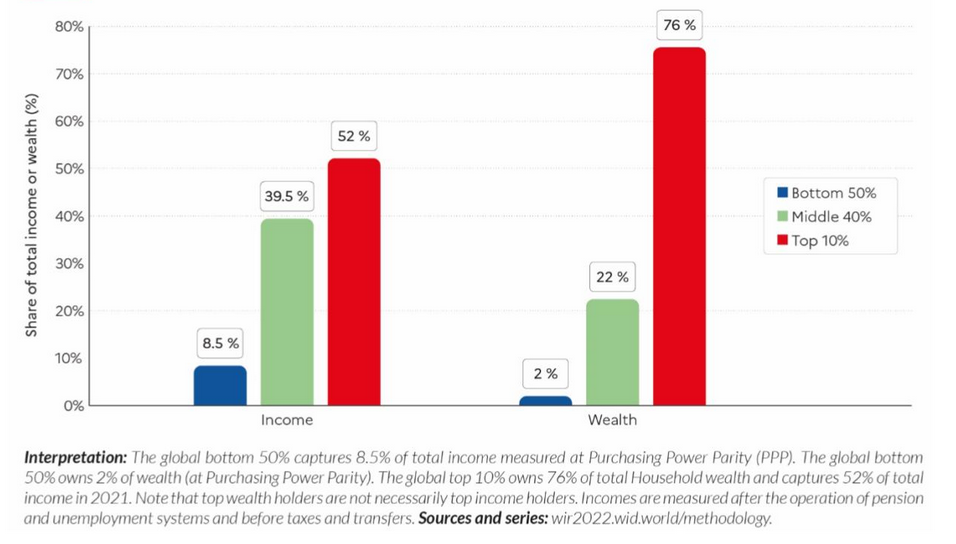
\includegraphics[width=1\linewidth]{images/11-income-versus-wealth.png}
	 	\caption{Global income and wealth inequality, 2021}
	 	\label{fig:income-versus-wealth}
	 \end{figure}
	
	The last main driver is \textbf{environmental and climate disruption}. The world's poorest people live in the most difficult environmental conditions. At the same time, the world’s poorest are highly dependent on their natural environment (like forest, grazing land, or water). On top of this material vulnerability comes the weak political and legal status of the poor. They often have no legal protection and no voice, which leaves them powerless against environmental crimes by large corporations, or even against their own government. Climate change reinforces the environmental damage. The annual damage from environmental disasters such as hurricanes, forest fires, droughts and floods already runs into tens of billions, and the bulk of that loss is suffered by the lowest-income groups, especially farmers. According to the UN, by 2030 already, climate warming would lead to an increase in extreme poverty by at least 120 million people.	
	\newpage
	\subsection{Concerns about inequality}
	
	The mere ethics are not the only reason why we should be concerned about inequality. There is also a link with human rights, economic development, environmental sustainability, societal well-being and political stability.
	\\\\
	First and foremost, we should recall that the Sustainable Development Goals are rooted in \textbf{human rights}. For a lot of SDGs, there is a one-to-one relationship with articles from the Universal Declaration of Human Rights. Malnutrition, child mortality and suicides of bankrupt farmers are clear indications that these rights are far from being realised. Eradicating extreme poverty is therefore rightly the very first SDG.
	\\\\
	Moreover, it is worth emphasizing that inequality and poverty are cross-cutting issues in all other global sustainability areas. \textbf{In addition to the economic realm (income, work, tax policies, international trade etc.) there are clear links with all dimensions of social life (education, healthcare, social participation, political voice) as well as with all planetary challenges (energy, natural resources, the environment and climate change).}
	\\\\
	Based on extensive statistical analysis of correlations between indicators of income inequality and indicators of unwellness in western societies, Wilkinson and Pickett claim in their famous publication ‘The spirit level’ that inequality is not only a problem of the victims, but of the whole population. More inequality has an impact on the \textbf{societal well-being} and is associated with lower social mobility, more crime, less confidence, poorer physical and mental health of the population, up to and including more addiction problems. The authors stress that even individuals from affluent groups suffer to some extent from inequality. They attribute this to socio-psychological effects such as stronger feelings of insecurity, of status competition, fear of being judged negatively by others, and a lower sense of belonging.
	\\\\
	Finally, inequality poses a threat to \textbf{political sustainability}. The increasing concentration of capital (and related power) in the hands of super-rich people poses a serious threat to democracy. Indeed, one cannot expect all super-rich to act ethically pure.
	
	\subsection{Policy solutions}
	
	A first solution relates to fairer globalization. Remarkably, Oxfam, the leading non-governmental actor in the development debate, does not argue against free trade but for fairer free trade. In doing so, Oxfam challenged the EU to further reduce its own import tariffs and export subsidies towards developing countries. Fair free trade even implies that poor countries should retain the right to protect weak sectors as long as necessary to prepare them for international competition. The use of fair trade labels helps to inform consumers on the ethical aspects of international trade. 
	\\\\
	The second policy strand deals with capital markets. Piketty's wants to combat extreme concentration of wealth. A key tool for this is a progressive tax on big fortunes. In the past decades, large-scale tax evasion by the most wealthy people as well as multinational had become a genuine plague. Thanks to multilateral agreements on the exchange of financial information, governments are beginning to get a grip on big wealth, and the feasibility of wealth taxation is increasing.
	\\\\
	A third set of policy prescriptions relates to the environmental and climate agenda. Our review of determinants of inequality shows how closely that agenda is intertwined with global redistribution - or at least, preventing inequality from derailing. The World Bank, for example, has calculated that limiting climate warming to 1.5 rather than 2 degrees could save hundreds of millions of people from poverty. Obviously, achieving this objective through ‘climate adaptation’ does come at a cost, which needs to be financed in a fair and solidary way.
	\\\\
	In addition to global-level strategies, more fine-grained and targeted strategies are of course also needed. The basic needs strategy focuses on the implementation of all the basic rights that the SDGs also refer to: right to food and water, health care, education, decent work and so on. Education has a particularly high social and economic return in developing countries, as it not only provides useful knowledge for the farm or labour market, but also `life skills' that contribute to better health, social cohesion, gender equality, civic responsibility and democracy. Summing up The combination of the above strategies soon brings us close to Kate Raworth's `doughnut economy'.
	
	\subsection{Kate Raworth's model of the doughnut economy}
	
	Kate Raworth does away with the dogma of endless linear growth. She advocates a circular economy that, while growing according to human needs, remains within the limits of what the planet can handle. In the image of the doughnut (see Figure \ref{fig:donut-economy}), the inner circle refers to the minimum prosperity needed to guarantee the basic rights of every human being (food, housing, education, health, social participation and so on), while the outer circle represents the maximum limits of planetary sustainability. The key, therefore, is to keep the economy in balance between these minimum and maximum limits. The basic circular pattern of the economy seeks to ensure that any form of `waste' can be reused, in order to spare the environment and climate.
	
	 \begin{figure}[htbp]
		\centering
		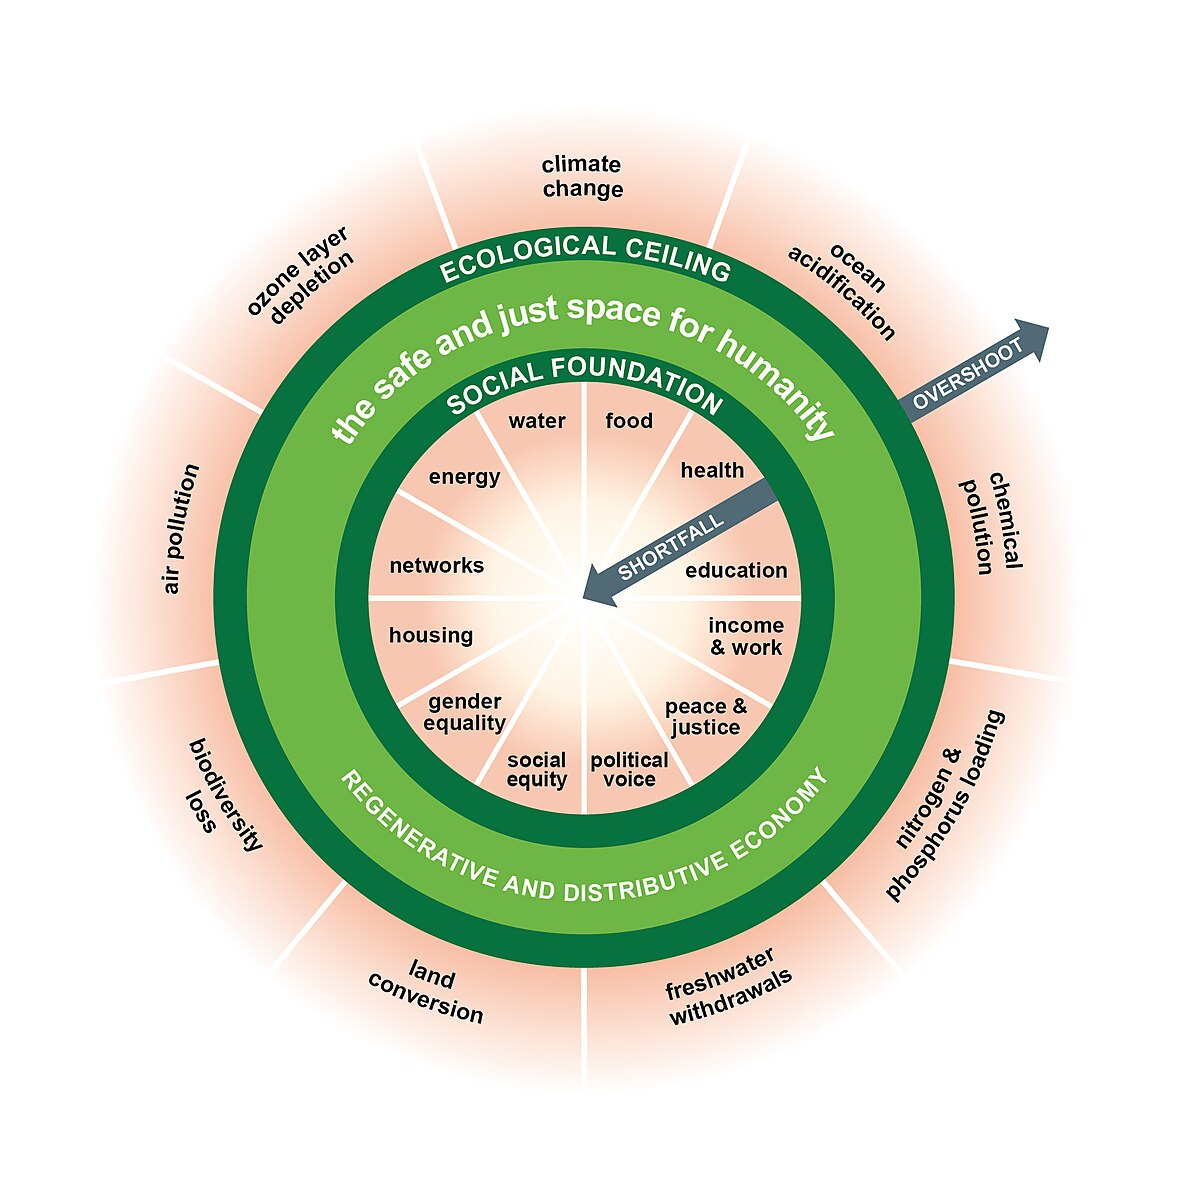
\includegraphics[width=1\linewidth]{images/11-donut-economy.png}
		\caption{Kate Raworth's model of the doughnut economy}
		\label{fig:donut-economy}
	\end{figure}
	
\end{document}